% This file is generated by the MATLAB m-file laprint.m. It can be included
% into LaTeX documents using the packages graphicx, color and psfrag.
% It is accompanied by a postscript file. A sample LaTeX file is:
%    \documentclass{article}\usepackage{graphicx,color,psfrag}
%    \begin{document}% This file is generated by the MATLAB m-file laprint.m. It can be included
% into LaTeX documents using the packages graphicx, color and psfrag.
% It is accompanied by a postscript file. A sample LaTeX file is:
%    \documentclass{article}\usepackage{graphicx,color,psfrag}
%    \begin{document}% This file is generated by the MATLAB m-file laprint.m. It can be included
% into LaTeX documents using the packages graphicx, color and psfrag.
% It is accompanied by a postscript file. A sample LaTeX file is:
%    \documentclass{article}\usepackage{graphicx,color,psfrag}
%    \begin{document}% This file is generated by the MATLAB m-file laprint.m. It can be included
% into LaTeX documents using the packages graphicx, color and psfrag.
% It is accompanied by a postscript file. A sample LaTeX file is:
%    \documentclass{article}\usepackage{graphicx,color,psfrag}
%    \begin{document}\input{Hellings_Downs}\end{document}
% See http://www.mathworks.de/matlabcentral/fileexchange/loadFile.do?objectId=4638
% for recent versions of laprint.m.
%
% created by:           LaPrint version 3.16 (13.9.2004)
% created on:           06-Aug-2014 15:59:04
% eps bounding box:     15 cm x 11.25 cm
% comment:              
%
\begin{psfrags}%
\psfragscanon%
%
% text strings:
\psfrag{s03}[t][t]{\color[rgb]{0,0,0}\setlength{\tabcolsep}{0pt}\begin{tabular}{c}\Large{}Angular separation $\theta/\mathrm{deg}$\end{tabular}}%
\psfrag{s04}[b][b]{\color[rgb]{0,0,0}\setlength{\tabcolsep}{0pt}\begin{tabular}{c}\Large{}Correlation $\Gamma_0$\end{tabular}}%
%
% xticklabels:
\psfrag{x01}[t][t]{$0$}%
\psfrag{x02}[t][t]{$20$}%
\psfrag{x03}[t][t]{$40$}%
\psfrag{x04}[t][t]{$60$}%
\psfrag{x05}[t][t]{$80$}%
\psfrag{x06}[t][t]{$100$}%
\psfrag{x07}[t][t]{$120$}%
\psfrag{x08}[t][t]{$140$}%
\psfrag{x09}[t][t]{$160$}%
\psfrag{x10}[t][t]{$180$}%
%
% yticklabels:
\psfrag{v01}[r][r]{$-0.2$}%
\psfrag{v02}[r][r]{$-0.1$}%
\psfrag{v03}[r][r]{$0.0$}%
\psfrag{v04}[r][r]{$0.1$}%
\psfrag{v05}[r][r]{$0.2$}%
\psfrag{v06}[r][r]{$0.3$}%
\psfrag{v07}[r][r]{$0.4$}%
\psfrag{v08}[r][r]{$0.5$}%
\psfrag{v09}[r][r]{$0.6$}%
%
% Figure:
\resizebox{12cm}{!}{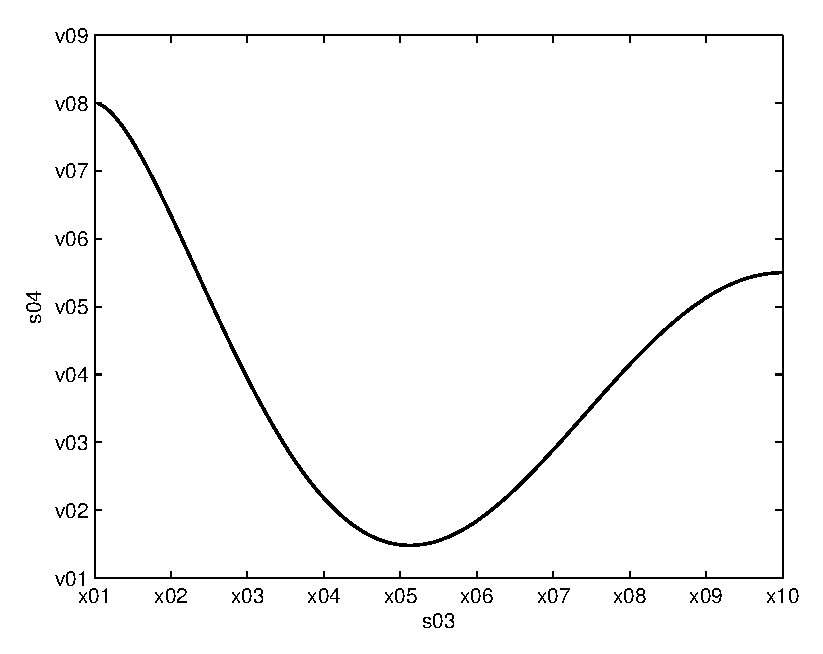
\includegraphics{Hellings_Downs.eps}}%
\end{psfrags}%
%
% End Hellings_Downs.tex
\end{document}
% See http://www.mathworks.de/matlabcentral/fileexchange/loadFile.do?objectId=4638
% for recent versions of laprint.m.
%
% created by:           LaPrint version 3.16 (13.9.2004)
% created on:           06-Aug-2014 15:59:04
% eps bounding box:     15 cm x 11.25 cm
% comment:              
%
\begin{psfrags}%
\psfragscanon%
%
% text strings:
\psfrag{s03}[t][t]{\color[rgb]{0,0,0}\setlength{\tabcolsep}{0pt}\begin{tabular}{c}\Large{}Angular separation $\theta/\mathrm{deg}$\end{tabular}}%
\psfrag{s04}[b][b]{\color[rgb]{0,0,0}\setlength{\tabcolsep}{0pt}\begin{tabular}{c}\Large{}Correlation $\Gamma_0$\end{tabular}}%
%
% xticklabels:
\psfrag{x01}[t][t]{$0$}%
\psfrag{x02}[t][t]{$20$}%
\psfrag{x03}[t][t]{$40$}%
\psfrag{x04}[t][t]{$60$}%
\psfrag{x05}[t][t]{$80$}%
\psfrag{x06}[t][t]{$100$}%
\psfrag{x07}[t][t]{$120$}%
\psfrag{x08}[t][t]{$140$}%
\psfrag{x09}[t][t]{$160$}%
\psfrag{x10}[t][t]{$180$}%
%
% yticklabels:
\psfrag{v01}[r][r]{$-0.2$}%
\psfrag{v02}[r][r]{$-0.1$}%
\psfrag{v03}[r][r]{$0.0$}%
\psfrag{v04}[r][r]{$0.1$}%
\psfrag{v05}[r][r]{$0.2$}%
\psfrag{v06}[r][r]{$0.3$}%
\psfrag{v07}[r][r]{$0.4$}%
\psfrag{v08}[r][r]{$0.5$}%
\psfrag{v09}[r][r]{$0.6$}%
%
% Figure:
\resizebox{12cm}{!}{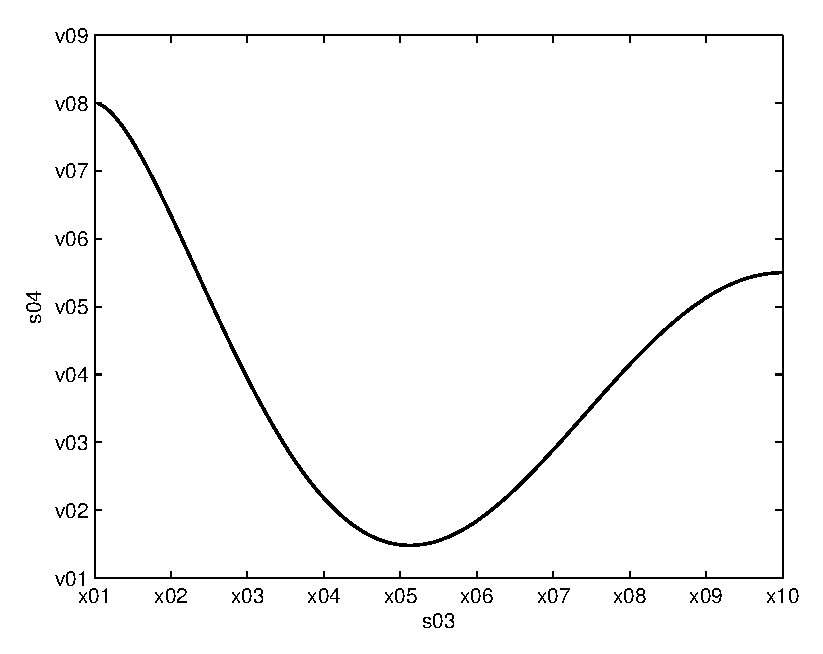
\includegraphics{Hellings_Downs.eps}}%
\end{psfrags}%
%
% End Hellings_Downs.tex
\end{document}
% See http://www.mathworks.de/matlabcentral/fileexchange/loadFile.do?objectId=4638
% for recent versions of laprint.m.
%
% created by:           LaPrint version 3.16 (13.9.2004)
% created on:           06-Aug-2014 15:59:04
% eps bounding box:     15 cm x 11.25 cm
% comment:              
%
\begin{psfrags}%
\psfragscanon%
%
% text strings:
\psfrag{s03}[t][t]{\color[rgb]{0,0,0}\setlength{\tabcolsep}{0pt}\begin{tabular}{c}\Large{}Angular separation $\theta/\mathrm{deg}$\end{tabular}}%
\psfrag{s04}[b][b]{\color[rgb]{0,0,0}\setlength{\tabcolsep}{0pt}\begin{tabular}{c}\Large{}Correlation $\Gamma_0$\end{tabular}}%
%
% xticklabels:
\psfrag{x01}[t][t]{$0$}%
\psfrag{x02}[t][t]{$20$}%
\psfrag{x03}[t][t]{$40$}%
\psfrag{x04}[t][t]{$60$}%
\psfrag{x05}[t][t]{$80$}%
\psfrag{x06}[t][t]{$100$}%
\psfrag{x07}[t][t]{$120$}%
\psfrag{x08}[t][t]{$140$}%
\psfrag{x09}[t][t]{$160$}%
\psfrag{x10}[t][t]{$180$}%
%
% yticklabels:
\psfrag{v01}[r][r]{$-0.2$}%
\psfrag{v02}[r][r]{$-0.1$}%
\psfrag{v03}[r][r]{$0.0$}%
\psfrag{v04}[r][r]{$0.1$}%
\psfrag{v05}[r][r]{$0.2$}%
\psfrag{v06}[r][r]{$0.3$}%
\psfrag{v07}[r][r]{$0.4$}%
\psfrag{v08}[r][r]{$0.5$}%
\psfrag{v09}[r][r]{$0.6$}%
%
% Figure:
\resizebox{12cm}{!}{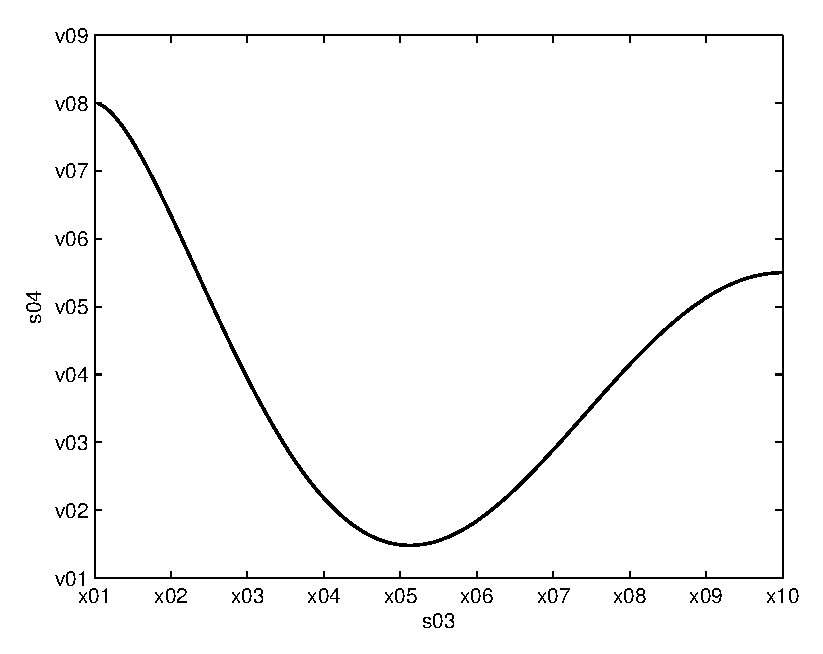
\includegraphics{Hellings_Downs.eps}}%
\end{psfrags}%
%
% End Hellings_Downs.tex
\end{document}
% See http://www.mathworks.de/matlabcentral/fileexchange/loadFile.do?objectId=4638
% for recent versions of laprint.m.
%
% created by:           LaPrint version 3.16 (13.9.2004)
% created on:           06-Aug-2014 15:59:04
% eps bounding box:     15 cm x 11.25 cm
% comment:              
%
\begin{psfrags}%
\psfragscanon%
%
% text strings:
\psfrag{s03}[t][t]{\color[rgb]{0,0,0}\setlength{\tabcolsep}{0pt}\begin{tabular}{c}\Large{}Angular separation $\theta/\mathrm{deg}$\end{tabular}}%
\psfrag{s04}[b][b]{\color[rgb]{0,0,0}\setlength{\tabcolsep}{0pt}\begin{tabular}{c}\Large{}Correlation $\Gamma_0$\end{tabular}}%
%
% xticklabels:
\psfrag{x01}[t][t]{$0$}%
\psfrag{x02}[t][t]{$20$}%
\psfrag{x03}[t][t]{$40$}%
\psfrag{x04}[t][t]{$60$}%
\psfrag{x05}[t][t]{$80$}%
\psfrag{x06}[t][t]{$100$}%
\psfrag{x07}[t][t]{$120$}%
\psfrag{x08}[t][t]{$140$}%
\psfrag{x09}[t][t]{$160$}%
\psfrag{x10}[t][t]{$180$}%
%
% yticklabels:
\psfrag{v01}[r][r]{$-0.2$}%
\psfrag{v02}[r][r]{$-0.1$}%
\psfrag{v03}[r][r]{$0.0$}%
\psfrag{v04}[r][r]{$0.1$}%
\psfrag{v05}[r][r]{$0.2$}%
\psfrag{v06}[r][r]{$0.3$}%
\psfrag{v07}[r][r]{$0.4$}%
\psfrag{v08}[r][r]{$0.5$}%
\psfrag{v09}[r][r]{$0.6$}%
%
% Figure:
\resizebox{12cm}{!}{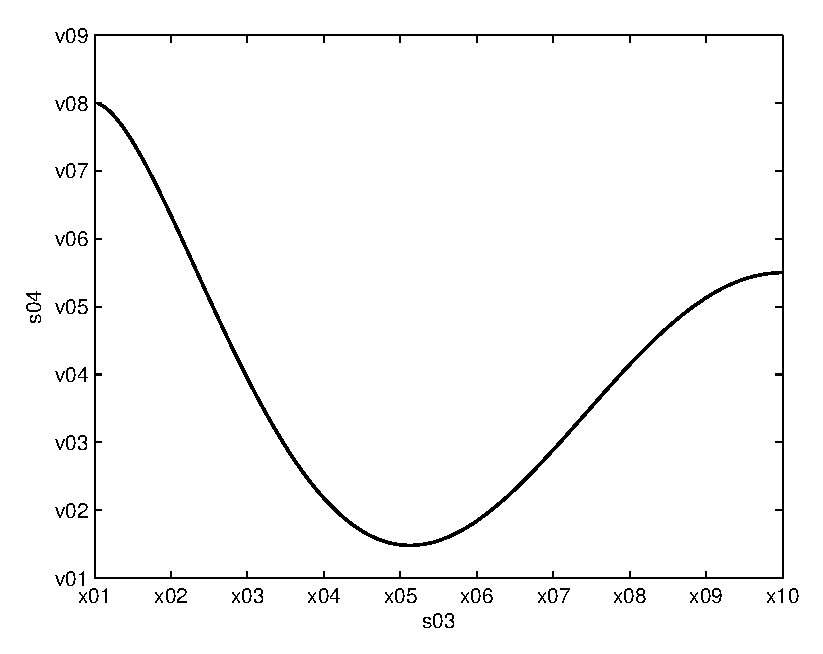
\includegraphics{Hellings_Downs.eps}}%
\end{psfrags}%
%
% End Hellings_Downs.tex
